\documentclass[1p]{elsarticle_modified}
%\bibliographystyle{elsarticle-num}

%\usepackage[colorlinks]{hyperref}
%\usepackage{abbrmath_seonhwa} %\Abb, \Ascr, \Acal ,\Abf, \Afrak
\usepackage{amsfonts}
\usepackage{amssymb}
\usepackage{amsmath}
\usepackage{amsthm}
\usepackage{scalefnt}
\usepackage{amsbsy}
\usepackage{kotex}
\usepackage{caption}
\usepackage{subfig}
\usepackage{color}
\usepackage{graphicx}
\usepackage{xcolor} %% white, black, red, green, blue, cyan, magenta, yellow
\usepackage{float}
\usepackage{setspace}
\usepackage{hyperref}

\usepackage{tikz}
\usetikzlibrary{arrows}

\usepackage{multirow}
\usepackage{array} % fixed length table
\usepackage{hhline}

%%%%%%%%%%%%%%%%%%%%%
\makeatletter
\renewcommand*\env@matrix[1][\arraystretch]{%
	\edef\arraystretch{#1}%
	\hskip -\arraycolsep
	\let\@ifnextchar\new@ifnextchar
	\array{*\c@MaxMatrixCols c}}
\makeatother %https://tex.stackexchange.com/questions/14071/how-can-i-increase-the-line-spacing-in-a-matrix
%%%%%%%%%%%%%%%

\usepackage[normalem]{ulem}

\newcommand{\msout}[1]{\ifmmode\text{\sout{\ensuremath{#1}}}\else\sout{#1}\fi}
%SOURCE: \msout is \stkout macro in https://tex.stackexchange.com/questions/20609/strikeout-in-math-mode

\newcommand{\cancel}[1]{
	\ifmmode
	{\color{red}\msout{#1}}
	\else
	{\color{red}\sout{#1}}
	\fi
}

\newcommand{\add}[1]{
	{\color{blue}\uwave{#1}}
}

\newcommand{\replace}[2]{
	\ifmmode
	{\color{red}\msout{#1}}{\color{blue}\uwave{#2}}
	\else
	{\color{red}\sout{#1}}{\color{blue}\uwave{#2}}
	\fi
}

\newcommand{\Sol}{\mathcal{S}} %segment
\newcommand{\D}{D} %diagram
\newcommand{\A}{\mathcal{A}} %arc


%%%%%%%%%%%%%%%%%%%%%%%%%%%%%5 test

\def\sl{\operatorname{\textup{SL}}(2,\Cbb)}
\def\psl{\operatorname{\textup{PSL}}(2,\Cbb)}
\def\quan{\mkern 1mu \triangleright \mkern 1mu}

\theoremstyle{definition}
\newtheorem{thm}{Theorem}[section]
\newtheorem{prop}[thm]{Proposition}
\newtheorem{lem}[thm]{Lemma}
\newtheorem{ques}[thm]{Question}
\newtheorem{cor}[thm]{Corollary}
\newtheorem{defn}[thm]{Definition}
\newtheorem{exam}[thm]{Example}
\newtheorem{rmk}[thm]{Remark}
\newtheorem{alg}[thm]{Algorithm}

\newcommand{\I}{\sqrt{-1}}
\begin{document}

%\begin{frontmatter}
%
%\title{Boundary parabolic representations of knots up to 8 crossings}
%
%%% Group authors per affiliation:
%\author{Yunhi Cho} 
%\address{Department of Mathematics, University of Seoul, Seoul, Korea}
%\ead{yhcho@uos.ac.kr}
%
%
%\author{Seonhwa Kim} %\fnref{s_kim}}
%\address{Center for Geometry and Physics, Institute for Basic Science, Pohang, 37673, Korea}
%\ead{ryeona17@ibs.re.kr}
%
%\author{Hyuk Kim}
%\address{Department of Mathematical Sciences, Seoul National University, Seoul 08826, Korea}
%\ead{hyukkim@snu.ac.kr}
%
%\author{Seokbeom Yoon}
%\address{Department of Mathematical Sciences, Seoul National University, Seoul, 08826,  Korea}
%\ead{sbyoon15@snu.ac.kr}
%
%\begin{abstract}
%We find all boundary parabolic representation of knots up to 8 crossings.
%
%\end{abstract}
%\begin{keyword}
%    \MSC[2010] 57M25 
%\end{keyword}
%
%\end{frontmatter}

%\linenumbers
%\tableofcontents
%
\newcommand\colored[1]{\textcolor{white}{\rule[-0.35ex]{0.8em}{1.4ex}}\kern-0.8em\color{red} #1}%
%\newcommand\colored[1]{\textcolor{white}{ #1}\kern-2.17ex	\textcolor{white}{ #1}\kern-1.81ex	\textcolor{white}{ #1}\kern-2.15ex\color{red}#1	}

{\Large $\underline{11a_{150}~(K11a_{150})}$}

\setlength{\tabcolsep}{10pt}
\renewcommand{\arraystretch}{1.6}
\vspace{1cm}\begin{tabular}{m{100pt}>{\centering\arraybackslash}m{274pt}}
\multirow{5}{120pt}{
	\centering
	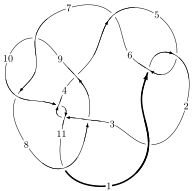
\includegraphics[width=112pt]{../../../GIT/diagram.site/Diagrams/png/399_11a_150.png}\\
\ \ \ A knot diagram\footnotemark}&
\allowdisplaybreaks
\textbf{Linearized knot diagam} \\
\cline{2-2}
 &
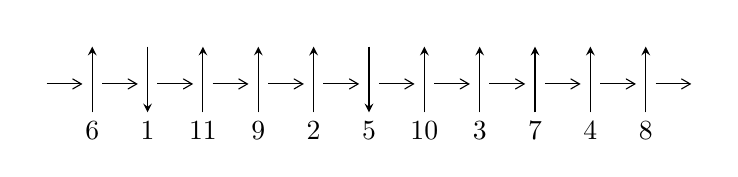
\begin{tikzpicture}[x=20pt, y=17pt]
	% nodes
	\node (C0) at (0, 0) {};
	\node (C1) at (1, 0) {};
	\node (C1U) at (1, +1) {};
	\node (C1D) at (1, -1) {6};

	\node (C2) at (2, 0) {};
	\node (C2U) at (2, +1) {};
	\node (C2D) at (2, -1) {1};

	\node (C3) at (3, 0) {};
	\node (C3U) at (3, +1) {};
	\node (C3D) at (3, -1) {11};

	\node (C4) at (4, 0) {};
	\node (C4U) at (4, +1) {};
	\node (C4D) at (4, -1) {9};

	\node (C5) at (5, 0) {};
	\node (C5U) at (5, +1) {};
	\node (C5D) at (5, -1) {2};

	\node (C6) at (6, 0) {};
	\node (C6U) at (6, +1) {};
	\node (C6D) at (6, -1) {5};

	\node (C7) at (7, 0) {};
	\node (C7U) at (7, +1) {};
	\node (C7D) at (7, -1) {10};

	\node (C8) at (8, 0) {};
	\node (C8U) at (8, +1) {};
	\node (C8D) at (8, -1) {3};

	\node (C9) at (9, 0) {};
	\node (C9U) at (9, +1) {};
	\node (C9D) at (9, -1) {7};

	\node (C10) at (10, 0) {};
	\node (C10U) at (10, +1) {};
	\node (C10D) at (10, -1) {4};

	\node (C11) at (11, 0) {};
	\node (C11U) at (11, +1) {};
	\node (C11D) at (11, -1) {8};
	\node (C12) at (12, 0) {};

	% arrows
	\draw[->,>={angle 60}]
	(C0) edge (C1) (C1) edge (C2) (C2) edge (C3) (C3) edge (C4) (C4) edge (C5) (C5) edge (C6) (C6) edge (C7) (C7) edge (C8) (C8) edge (C9) (C9) edge (C10) (C10) edge (C11) (C11) edge (C12) ;	\draw[->,>=stealth]
	(C1D) edge (C1U) (C2U) edge (C2D) (C3D) edge (C3U) (C4D) edge (C4U) (C5D) edge (C5U) (C6U) edge (C6D) (C7D) edge (C7U) (C8D) edge (C8U) (C9D) edge (C9U) (C10D) edge (C10U) (C11D) edge (C11U) ;
	\end{tikzpicture} \\
\hhline{~~} \\& 
\textbf{Solving Sequence} \\ \cline{2-2} 
 &
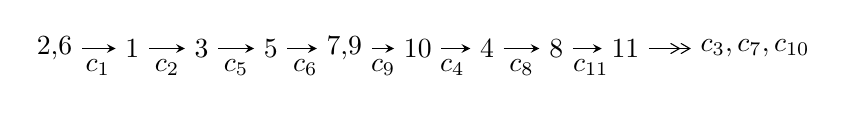
\begin{tikzpicture}[x=25pt, y=7pt]
	% node
	\node (A0) at (-1/8, 0) {2,6};
	\node (A1) at (1, 0) {1};
	\node (A2) at (2, 0) {3};
	\node (A3) at (3, 0) {5};
	\node (A4) at (65/16, 0) {7,9};
	\node (A5) at (41/8, 0) {10};
	\node (A6) at (49/8, 0) {4};
	\node (A7) at (57/8, 0) {8};
	\node (A8) at (65/8, 0) {11};
	\node (C1) at (1/2, -1) {$c_{1}$};
	\node (C2) at (3/2, -1) {$c_{2}$};
	\node (C3) at (5/2, -1) {$c_{5}$};
	\node (C4) at (7/2, -1) {$c_{6}$};
	\node (C5) at (37/8, -1) {$c_{9}$};
	\node (C6) at (45/8, -1) {$c_{4}$};
	\node (C7) at (53/8, -1) {$c_{8}$};
	\node (C8) at (61/8, -1) {$c_{11}$};
	\node (A9) at (10, 0) {$c_{3},c_{7},c_{10}$};

	% edge
	\draw[->,>=stealth]	
	(A0) edge (A1) (A1) edge (A2) (A2) edge (A3) (A3) edge (A4) (A4) edge (A5) (A5) edge (A6) (A6) edge (A7) (A7) edge (A8) ;
	\draw[->>,>={angle 60}]	
	(A8) edge (A9);
\end{tikzpicture} \\ 

\end{tabular} \\

\footnotetext{
The image of knot diagram is generated by the software ``\textbf{Draw programme}" developed by Andrew Bartholomew(\url{http://www.layer8.co.uk/maths/draw/index.htm\#Running-draw}), where we modified some parts for our purpose(\url{https://github.com/CATsTAILs/LinksPainter}).
}\phantom \\ \newline 
\centering \textbf{Ideals for irreducible components\footnotemark of $X_{\text{par}}$} 
 
\begin{align*}
I^u_{1}&=\langle 
5.92448\times10^{33} u^{61}-1.02898\times10^{34} u^{60}+\cdots+1.17126\times10^{34} b-5.31916\times10^{33},\\
\phantom{I^u_{1}}&\phantom{= \langle  }8.54907\times10^{32} u^{61}+2.67122\times10^{33} u^{60}+\cdots+1.17126\times10^{34} a-1.99667\times10^{34},\;u^{62}-3 u^{61}+\cdots-3 u+1\rangle \\
\\
\end{align*}
\raggedright * 1 irreducible components of $\dim_{\mathbb{C}}=0$, with total 62 representations.\\
\footnotetext{All coefficients of polynomials are rational numbers. But the coefficients are sometimes approximated in decimal forms when there is not enough margin.}
\newpage
\renewcommand{\arraystretch}{1}
\centering \section*{I. $I^u_{1}= \langle 5.92\times10^{33} u^{61}-1.03\times10^{34} u^{60}+\cdots+1.17\times10^{34} b-5.32\times10^{33},\;8.55\times10^{32} u^{61}+2.67\times10^{33} u^{60}+\cdots+1.17\times10^{34} a-2.00\times10^{34},\;u^{62}-3 u^{61}+\cdots-3 u+1 \rangle$}
\flushleft \textbf{(i) Arc colorings}\\
\begin{tabular}{m{7pt} m{180pt} m{7pt} m{180pt} }
\flushright $a_{2}=$&$\begin{pmatrix}1\\0\end{pmatrix}$ \\
\flushright $a_{6}=$&$\begin{pmatrix}0\\u\end{pmatrix}$ \\
\flushright $a_{1}=$&$\begin{pmatrix}1\\u^2\end{pmatrix}$ \\
\flushright $a_{3}=$&$\begin{pmatrix}u^2+1\\u^4\end{pmatrix}$ \\
\flushright $a_{5}=$&$\begin{pmatrix}- u\\u\end{pmatrix}$ \\
\flushright $a_{7}=$&$\begin{pmatrix}- u^3\\u^3+u\end{pmatrix}$ \\
\flushright $a_{9}=$&$\begin{pmatrix}-0.0729904 u^{61}-0.228063 u^{60}+\cdots-3.85257 u+1.70472\\-0.505821 u^{61}+0.878522 u^{60}+\cdots+0.946087 u+0.454140\end{pmatrix}$ \\
\flushright $a_{10}=$&$\begin{pmatrix}0.0556025 u^{61}-0.656967 u^{60}+\cdots-3.50832 u+1.53444\\-0.800994 u^{61}+1.63689 u^{60}+\cdots-0.390734 u+0.638367\end{pmatrix}$ \\
\flushright $a_{4}=$&$\begin{pmatrix}0.955009 u^{61}-3.66751 u^{60}+\cdots+4.99704 u-2.34895\\-0.104931 u^{61}+0.897107 u^{60}+\cdots+0.756639 u-0.648091\end{pmatrix}$ \\
\flushright $a_{8}=$&$\begin{pmatrix}-0.101533 u^{61}-0.116613 u^{60}+\cdots-5.40842 u+1.67042\\-0.557807 u^{61}+1.02766 u^{60}+\cdots+0.790291 u+0.499051\end{pmatrix}$ \\
\flushright $a_{11}=$&$\begin{pmatrix}-0.212577 u^{61}+0.857984 u^{60}+\cdots-5.64360 u+3.30260\\-1.52544 u^{61}+4.42060 u^{60}+\cdots+2.47746 u-0.957556\end{pmatrix}$\\ \flushright $a_{11}=$&$\begin{pmatrix}-0.212577 u^{61}+0.857984 u^{60}+\cdots-5.64360 u+3.30260\\-1.52544 u^{61}+4.42060 u^{60}+\cdots+2.47746 u-0.957556\end{pmatrix}$\\&\end{tabular}
\flushleft \textbf{(ii) Obstruction class $= -1$}\\~\\
\flushleft \textbf{(iii) Cusp Shapes $= -2.26821 u^{61}+7.95048 u^{60}+\cdots-1.19620 u+11.3832$}\\~\\
\newpage\renewcommand{\arraystretch}{1}
\flushleft \textbf{(iv) u-Polynomials at the component}\newline \\
\begin{tabular}{m{50pt}|m{274pt}}
Crossings & \hspace{64pt}u-Polynomials at each crossing \\
\hline $$\begin{aligned}c_{1},c_{5}\end{aligned}$$&$\begin{aligned}
&u^{62}-3 u^{61}+\cdots-3 u+1
\end{aligned}$\\
\hline $$\begin{aligned}c_{2},c_{6}\end{aligned}$$&$\begin{aligned}
&u^{62}+17 u^{61}+\cdots- u+1
\end{aligned}$\\
\hline $$\begin{aligned}c_{3},c_{10}\end{aligned}$$&$\begin{aligned}
&u^{62}+3 u^{61}+\cdots- u+1
\end{aligned}$\\
\hline $$\begin{aligned}c_{4}\end{aligned}$$&$\begin{aligned}
&u^{62}+15 u^{61}+\cdots+14601 u-4393
\end{aligned}$\\
\hline $$\begin{aligned}c_{7},c_{9}\end{aligned}$$&$\begin{aligned}
&u^{62}+u^{61}+\cdots+3 u-1
\end{aligned}$\\
\hline $$\begin{aligned}c_{8}\end{aligned}$$&$\begin{aligned}
&u^{62}+u^{61}+\cdots-11 u-1
\end{aligned}$\\
\hline $$\begin{aligned}c_{11}\end{aligned}$$&$\begin{aligned}
&u^{62}+27 u^{61}+\cdots-73 u-43
\end{aligned}$\\
\hline
\end{tabular}\\~\\
\newpage\renewcommand{\arraystretch}{1}
\flushleft \textbf{(v) Riley Polynomials at the component}\newline \\
\begin{tabular}{m{50pt}|m{274pt}}
Crossings & \hspace{64pt}Riley Polynomials at each crossing \\
\hline $$\begin{aligned}c_{1},c_{5}\end{aligned}$$&$\begin{aligned}
&y^{62}+17 y^{61}+\cdots- y+1
\end{aligned}$\\
\hline $$\begin{aligned}c_{2},c_{6}\end{aligned}$$&$\begin{aligned}
&y^{62}+57 y^{61}+\cdots-49 y+1
\end{aligned}$\\
\hline $$\begin{aligned}c_{3},c_{10}\end{aligned}$$&$\begin{aligned}
&y^{62}+37 y^{61}+\cdots- y+1
\end{aligned}$\\
\hline $$\begin{aligned}c_{4}\end{aligned}$$&$\begin{aligned}
&y^{62}+345 y^{61}+\cdots-184476553 y+19298449
\end{aligned}$\\
\hline $$\begin{aligned}c_{7},c_{9}\end{aligned}$$&$\begin{aligned}
&y^{62}-43 y^{61}+\cdots+67 y+1
\end{aligned}$\\
\hline $$\begin{aligned}c_{8}\end{aligned}$$&$\begin{aligned}
&y^{62}-3 y^{61}+\cdots+27 y+1
\end{aligned}$\\
\hline $$\begin{aligned}c_{11}\end{aligned}$$&$\begin{aligned}
&y^{62}-343 y^{61}+\cdots-98037 y+1849
\end{aligned}$\\
\hline
\end{tabular}\\~\\
\newpage\flushleft \textbf{(vi) Complex Volumes and Cusp Shapes}
$$\begin{array}{c|c|c}  
\text{Solutions to }I^u_{1}& \I (\text{vol} + \sqrt{-1}CS) & \text{Cusp shape}\\
 \hline 
\begin{aligned}
u &= -0.233941 + 0.974873 I \\
a &= -0.130745 + 1.231300 I \\
b &= \phantom{-}1.20344 - 0.93140 I\end{aligned}
 & -5.58386 - 5.07710 I & \phantom{-0.000000 -}0. + 6.39246 I \\ \hline\begin{aligned}
u &= -0.233941 - 0.974873 I \\
a &= -0.130745 - 1.231300 I \\
b &= \phantom{-}1.20344 + 0.93140 I\end{aligned}
 & -5.58386 + 5.07710 I & \phantom{-0.000000 } 0. - 6.39246 I \\ \hline\begin{aligned}
u &= -0.342652 + 0.944226 I \\
a &= -0.419993 - 0.060562 I \\
b &= -0.625287 + 0.596594 I\end{aligned}
 & -5.00545 - 0.49255 I & \phantom{-0.000000 -}0. + 3.20018 I \\ \hline\begin{aligned}
u &= -0.342652 - 0.944226 I \\
a &= -0.419993 + 0.060562 I \\
b &= -0.625287 - 0.596594 I\end{aligned}
 & -5.00545 + 0.49255 I & \phantom{-0.000000 } 0. - 3.20018 I \\ \hline\begin{aligned}
u &= \phantom{-}0.153290 + 0.920392 I \\
a &= \phantom{-}0.174303 + 0.695564 I \\
b &= -0.725323 - 0.206126 I\end{aligned}
 & -1.76466 + 1.66966 I & \phantom{-}2.52149 - 4.58368 I \\ \hline\begin{aligned}
u &= \phantom{-}0.153290 - 0.920392 I \\
a &= \phantom{-}0.174303 - 0.695564 I \\
b &= -0.725323 + 0.206126 I\end{aligned}
 & -1.76466 - 1.66966 I & \phantom{-}2.52149 + 4.58368 I \\ \hline\begin{aligned}
u &= \phantom{-}0.929527\phantom{ +0.000000I} \\
a &= -0.431713\phantom{ +0.000000I} \\
b &= -0.530504\phantom{ +0.000000I}\end{aligned}
 & \phantom{-}4.73356\phantom{ +0.000000I} & \phantom{-}21.5180\phantom{ +0.000000I} \\ \hline\begin{aligned}
u &= \phantom{-}0.736100 + 0.839352 I \\
a &= \phantom{-}0.625972 - 1.122520 I \\
b &= \phantom{-}0.25553 + 1.54232 I\end{aligned}
 & \phantom{-}1.37977 + 2.70121 I & \phantom{-0.000000 } 0 \\ \hline\begin{aligned}
u &= \phantom{-}0.736100 - 0.839352 I \\
a &= \phantom{-}0.625972 + 1.122520 I \\
b &= \phantom{-}0.25553 - 1.54232 I\end{aligned}
 & \phantom{-}1.37977 - 2.70121 I & \phantom{-0.000000 } 0 \\ \hline\begin{aligned}
u &= -0.789702 + 0.810743 I \\
a &= \phantom{-}1.12489 - 1.57251 I \\
b &= -1.73762 + 0.87825 I\end{aligned}
 & \phantom{-}4.18121 - 0.02705 I & \phantom{-0.000000 } 0\\
 \hline 
 \end{array}$$\newpage$$\begin{array}{c|c|c}  
\text{Solutions to }I^u_{1}& \I (\text{vol} + \sqrt{-1}CS) & \text{Cusp shape}\\
 \hline 
\begin{aligned}
u &= -0.789702 - 0.810743 I \\
a &= \phantom{-}1.12489 + 1.57251 I \\
b &= -1.73762 - 0.87825 I\end{aligned}
 & \phantom{-}4.18121 + 0.02705 I & \phantom{-0.000000 } 0 \\ \hline\begin{aligned}
u &= \phantom{-}0.817053 + 0.788358 I \\
a &= -1.72604 - 1.05558 I \\
b &= \phantom{-}1.91057 + 0.30098 I\end{aligned}
 & \phantom{-}1.14770 - 3.66515 I & \phantom{-0.000000 } 0 \\ \hline\begin{aligned}
u &= \phantom{-}0.817053 - 0.788358 I \\
a &= -1.72604 + 1.05558 I \\
b &= \phantom{-}1.91057 - 0.30098 I\end{aligned}
 & \phantom{-}1.14770 + 3.66515 I & \phantom{-0.000000 } 0 \\ \hline\begin{aligned}
u &= -0.330897 + 1.086980 I \\
a &= \phantom{-}0.052301 - 0.533925 I \\
b &= -1.136400 - 0.072139 I\end{aligned}
 & -2.42165 - 10.69330 I & \phantom{-0.000000 } 0 \\ \hline\begin{aligned}
u &= -0.330897 - 1.086980 I \\
a &= \phantom{-}0.052301 + 0.533925 I \\
b &= -1.136400 + 0.072139 I\end{aligned}
 & -2.42165 + 10.69330 I & \phantom{-0.000000 } 0 \\ \hline\begin{aligned}
u &= -0.191245 + 1.125970 I \\
a &= \phantom{-}0.424086 + 0.452072 I \\
b &= -0.112808 - 0.950910 I\end{aligned}
 & -3.25243 + 3.43205 I & \phantom{-0.000000 } 0 \\ \hline\begin{aligned}
u &= -0.191245 - 1.125970 I \\
a &= \phantom{-}0.424086 - 0.452072 I \\
b &= -0.112808 + 0.950910 I\end{aligned}
 & -3.25243 - 3.43205 I & \phantom{-0.000000 } 0 \\ \hline\begin{aligned}
u &= \phantom{-}0.699940 + 0.915282 I \\
a &= \phantom{-}0.883343 + 0.109262 I \\
b &= -0.665362 + 0.493910 I\end{aligned}
 & \phantom{-}1.15333 + 2.78689 I & \phantom{-0.000000 } 0 \\ \hline\begin{aligned}
u &= \phantom{-}0.699940 - 0.915282 I \\
a &= \phantom{-}0.883343 - 0.109262 I \\
b &= -0.665362 - 0.493910 I\end{aligned}
 & \phantom{-}1.15333 - 2.78689 I & \phantom{-0.000000 } 0 \\ \hline\begin{aligned}
u &= \phantom{-}0.293896 + 0.791599 I \\
a &= \phantom{-}1.372560 - 0.140152 I \\
b &= -1.74453 + 0.97363 I\end{aligned}
 & -0.39022 + 3.86672 I & \phantom{-}5.90788 - 9.08899 I\\
 \hline 
 \end{array}$$\newpage$$\begin{array}{c|c|c}  
\text{Solutions to }I^u_{1}& \I (\text{vol} + \sqrt{-1}CS) & \text{Cusp shape}\\
 \hline 
\begin{aligned}
u &= \phantom{-}0.293896 - 0.791599 I \\
a &= \phantom{-}1.372560 + 0.140152 I \\
b &= -1.74453 - 0.97363 I\end{aligned}
 & -0.39022 - 3.86672 I & \phantom{-}5.90788 + 9.08899 I \\ \hline\begin{aligned}
u &= -0.751244 + 0.881873 I \\
a &= \phantom{-}7.9454 + 16.0972 I \\
b &= \phantom{-}5.3873 - 20.3768 I\end{aligned}
 & \phantom{-}3.03672 - 2.84894 I & -90.977 - 147.127 I \\ \hline\begin{aligned}
u &= -0.751244 - 0.881873 I \\
a &= \phantom{-}7.9454 - 16.0972 I \\
b &= \phantom{-}5.3873 + 20.3768 I\end{aligned}
 & \phantom{-}3.03672 + 2.84894 I & -90.977 + 147.127 I \\ \hline\begin{aligned}
u &= \phantom{-}0.099206 + 0.819273 I \\
a &= -0.693059 + 0.958627 I \\
b &= -0.97879 + 1.67339 I\end{aligned}
 & -1.49291 - 0.30288 I & \phantom{-}6.68102 - 7.18270 I \\ \hline\begin{aligned}
u &= \phantom{-}0.099206 - 0.819273 I \\
a &= -0.693059 - 0.958627 I \\
b &= -0.97879 - 1.67339 I\end{aligned}
 & -1.49291 + 0.30288 I & \phantom{-}6.68102 + 7.18270 I \\ \hline\begin{aligned}
u &= -0.811325 + 0.855337 I \\
a &= \phantom{-}1.02748 - 1.98302 I \\
b &= -1.43041 + 0.97746 I\end{aligned}
 & \phantom{-}5.99939 + 0.78225 I & \phantom{-0.000000 } 0 \\ \hline\begin{aligned}
u &= -0.811325 - 0.855337 I \\
a &= \phantom{-}1.02748 + 1.98302 I \\
b &= -1.43041 - 0.97746 I\end{aligned}
 & \phantom{-}5.99939 - 0.78225 I & \phantom{-0.000000 } 0 \\ \hline\begin{aligned}
u &= -0.817162 + 0.076718 I \\
a &= \phantom{-}0.557951 + 0.249895 I \\
b &= \phantom{-}0.619554 + 0.545965 I\end{aligned}
 & \phantom{-}0.96723 + 6.76946 I & \phantom{-}10.42875 - 6.10913 I \\ \hline\begin{aligned}
u &= -0.817162 - 0.076718 I \\
a &= \phantom{-}0.557951 - 0.249895 I \\
b &= \phantom{-}0.619554 - 0.545965 I\end{aligned}
 & \phantom{-}0.96723 - 6.76946 I & \phantom{-}10.42875 + 6.10913 I \\ \hline\begin{aligned}
u &= \phantom{-}0.903335 + 0.763131 I \\
a &= \phantom{-}1.58371 + 1.40581 I \\
b &= -2.04345 + 0.10821 I\end{aligned}
 & \phantom{-}5.82273 - 9.92532 I & \phantom{-0.000000 } 0\\
 \hline 
 \end{array}$$\newpage$$\begin{array}{c|c|c}  
\text{Solutions to }I^u_{1}& \I (\text{vol} + \sqrt{-1}CS) & \text{Cusp shape}\\
 \hline 
\begin{aligned}
u &= \phantom{-}0.903335 - 0.763131 I \\
a &= \phantom{-}1.58371 - 1.40581 I \\
b &= -2.04345 - 0.10821 I\end{aligned}
 & \phantom{-}5.82273 + 9.92532 I & \phantom{-0.000000 } 0 \\ \hline\begin{aligned}
u &= \phantom{-}0.801297 + 0.878767 I \\
a &= -0.483885 - 0.937624 I \\
b &= \phantom{-}0.274288 + 0.065829 I\end{aligned}
 & \phantom{-}6.91724 + 2.74492 I & \phantom{-0.000000 } 0 \\ \hline\begin{aligned}
u &= \phantom{-}0.801297 - 0.878767 I \\
a &= -0.483885 + 0.937624 I \\
b &= \phantom{-}0.274288 - 0.065829 I\end{aligned}
 & \phantom{-}6.91724 - 2.74492 I & \phantom{-0.000000 } 0 \\ \hline\begin{aligned}
u &= -0.919899 + 0.762554 I \\
a &= -1.09122 + 1.22881 I \\
b &= \phantom{-}1.52740 - 0.02797 I\end{aligned}
 & \phantom{-}9.64228 + 3.86851 I & \phantom{-0.000000 } 0 \\ \hline\begin{aligned}
u &= -0.919899 - 0.762554 I \\
a &= -1.09122 - 1.22881 I \\
b &= \phantom{-}1.52740 + 0.02797 I\end{aligned}
 & \phantom{-}9.64228 - 3.86851 I & \phantom{-0.000000 } 0 \\ \hline\begin{aligned}
u &= \phantom{-}0.384411 + 1.134740 I \\
a &= -0.110043 - 0.199538 I \\
b &= \phantom{-}0.727530 - 0.187535 I\end{aligned}
 & \phantom{-}0.94109 + 4.46712 I & \phantom{-0.000000 } 0 \\ \hline\begin{aligned}
u &= \phantom{-}0.384411 - 1.134740 I \\
a &= -0.110043 + 0.199538 I \\
b &= \phantom{-}0.727530 + 0.187535 I\end{aligned}
 & \phantom{-}0.94109 - 4.46712 I & \phantom{-0.000000 } 0 \\ \hline\begin{aligned}
u &= \phantom{-}0.794631 + 0.900072 I \\
a &= \phantom{-}0.529387 + 0.334235 I \\
b &= -1.36232 - 0.59261 I\end{aligned}
 & \phantom{-}6.85084 + 3.23980 I & \phantom{-0.000000 } 0 \\ \hline\begin{aligned}
u &= \phantom{-}0.794631 - 0.900072 I \\
a &= \phantom{-}0.529387 - 0.334235 I \\
b &= -1.36232 + 0.59261 I\end{aligned}
 & \phantom{-}6.85084 - 3.23980 I & \phantom{-0.000000 } 0 \\ \hline\begin{aligned}
u &= -0.758229 + 0.946770 I \\
a &= -1.32947 + 1.46124 I \\
b &= \phantom{-}2.03631 - 0.87059 I\end{aligned}
 & \phantom{-}3.76313 - 5.80968 I & \phantom{-0.000000 } 0\\
 \hline 
 \end{array}$$\newpage$$\begin{array}{c|c|c}  
\text{Solutions to }I^u_{1}& \I (\text{vol} + \sqrt{-1}CS) & \text{Cusp shape}\\
 \hline 
\begin{aligned}
u &= -0.758229 - 0.946770 I \\
a &= -1.32947 - 1.46124 I \\
b &= \phantom{-}2.03631 + 0.87059 I\end{aligned}
 & \phantom{-}3.76313 + 5.80968 I & \phantom{-0.000000 } 0 \\ \hline\begin{aligned}
u &= -0.792260 + 0.922878 I \\
a &= -1.64621 + 1.05149 I \\
b &= \phantom{-}2.57092 - 0.66498 I\end{aligned}
 & \phantom{-}5.79100 - 6.78973 I & \phantom{-0.000000 } 0 \\ \hline\begin{aligned}
u &= -0.792260 - 0.922878 I \\
a &= -1.64621 - 1.05149 I \\
b &= \phantom{-}2.57092 + 0.66498 I\end{aligned}
 & \phantom{-}5.79100 + 6.78973 I & \phantom{-0.000000 } 0 \\ \hline\begin{aligned}
u &= \phantom{-}0.989705 + 0.719878 I \\
a &= \phantom{-}0.244303 + 0.652654 I \\
b &= -0.528313 - 0.037104 I\end{aligned}
 & \phantom{-}4.58484 + 2.57158 I & \phantom{-0.000000 } 0 \\ \hline\begin{aligned}
u &= \phantom{-}0.989705 - 0.719878 I \\
a &= \phantom{-}0.244303 - 0.652654 I \\
b &= -0.528313 + 0.037104 I\end{aligned}
 & \phantom{-}4.58484 - 2.57158 I & \phantom{-0.000000 } 0 \\ \hline\begin{aligned}
u &= \phantom{-}0.767748 + 0.968583 I \\
a &= \phantom{-}0.93996 + 1.97333 I \\
b &= -1.74350 - 1.71204 I\end{aligned}
 & \phantom{-}0.59571 + 9.61001 I & \phantom{-0.000000 } 0 \\ \hline\begin{aligned}
u &= \phantom{-}0.767748 - 0.968583 I \\
a &= \phantom{-}0.93996 - 1.97333 I \\
b &= -1.74350 + 1.71204 I\end{aligned}
 & \phantom{-}0.59571 - 9.61001 I & \phantom{-0.000000 } 0 \\ \hline\begin{aligned}
u &= \phantom{-}0.796750 + 1.019410 I \\
a &= -1.09739 - 1.94527 I \\
b &= \phantom{-}2.54984 + 1.54483 I\end{aligned}
 & \phantom{-}5.0175 + 16.2111 I & \phantom{-0.000000 } 0 \\ \hline\begin{aligned}
u &= \phantom{-}0.796750 - 1.019410 I \\
a &= -1.09739 + 1.94527 I \\
b &= \phantom{-}2.54984 - 1.54483 I\end{aligned}
 & \phantom{-}5.0175 - 16.2111 I & \phantom{-0.000000 } 0 \\ \hline\begin{aligned}
u &= -0.208653 + 0.671289 I \\
a &= -0.50660 - 1.40640 I \\
b &= \phantom{-}0.966809 + 0.993102 I\end{aligned}
 & \phantom{-}1.24146 - 0.98622 I & \phantom{-}9.68923 - 0.00108 I\\
 \hline 
 \end{array}$$\newpage$$\begin{array}{c|c|c}  
\text{Solutions to }I^u_{1}& \I (\text{vol} + \sqrt{-1}CS) & \text{Cusp shape}\\
 \hline 
\begin{aligned}
u &= -0.208653 - 0.671289 I \\
a &= -0.50660 + 1.40640 I \\
b &= \phantom{-}0.966809 - 0.993102 I\end{aligned}
 & \phantom{-}1.24146 + 0.98622 I & \phantom{-}9.68923 + 0.00108 I \\ \hline\begin{aligned}
u &= -0.804538 + 1.026660 I \\
a &= \phantom{-}0.95806 - 1.42226 I \\
b &= -2.12242 + 1.08518 I\end{aligned}
 & \phantom{-}8.80960 - 10.22650 I & \phantom{-0.000000 } 0 \\ \hline\begin{aligned}
u &= -0.804538 - 1.026660 I \\
a &= \phantom{-}0.95806 + 1.42226 I \\
b &= -2.12242 - 1.08518 I\end{aligned}
 & \phantom{-}8.80960 + 10.22650 I & \phantom{-0.000000 } 0 \\ \hline\begin{aligned}
u &= \phantom{-}0.852377 + 1.058720 I \\
a &= -0.240483 - 0.650672 I \\
b &= \phantom{-}0.924864 + 0.679823 I\end{aligned}
 & \phantom{-}3.54226 + 4.13545 I & \phantom{-0.000000 } 0 \\ \hline\begin{aligned}
u &= \phantom{-}0.852377 - 1.058720 I \\
a &= -0.240483 + 0.650672 I \\
b &= \phantom{-}0.924864 - 0.679823 I\end{aligned}
 & \phantom{-}3.54226 - 4.13545 I & \phantom{-0.000000 } 0 \\ \hline\begin{aligned}
u &= -0.267685 + 0.530806 I \\
a &= -1.06202 - 2.33490 I \\
b &= \phantom{-}0.263606 + 1.305770 I\end{aligned}
 & \phantom{-}1.46923 - 1.18627 I & \phantom{-}9.25634 + 4.59290 I \\ \hline\begin{aligned}
u &= -0.267685 - 0.530806 I \\
a &= -1.06202 + 2.33490 I \\
b &= \phantom{-}0.263606 - 1.305770 I\end{aligned}
 & \phantom{-}1.46923 + 1.18627 I & \phantom{-}9.25634 - 4.59290 I \\ \hline\begin{aligned}
u &= -0.535919 + 0.048687 I \\
a &= \phantom{-}0.045166 + 0.921741 I \\
b &= -0.559745 + 0.668972 I\end{aligned}
 & -2.56130 - 2.50988 I & \phantom{-}6.34359 + 3.13989 I \\ \hline\begin{aligned}
u &= -0.535919 - 0.048687 I \\
a &= \phantom{-}0.045166 - 0.921741 I \\
b &= -0.559745 - 0.668972 I\end{aligned}
 & -2.56130 + 2.50988 I & \phantom{-}6.34359 - 3.13989 I \\ \hline\begin{aligned}
u &= \phantom{-}0.335461 + 0.238621 I \\
a &= \phantom{-}1.34053 - 2.57954 I \\
b &= \phantom{-}0.814929 + 0.614489 I\end{aligned}
 & \phantom{-}1.04914 - 1.31929 I & \phantom{-}11.02923 + 0.35157 I\\
 \hline 
 \end{array}$$\newpage$$\begin{array}{c|c|c}  
\text{Solutions to }I^u_{1}& \I (\text{vol} + \sqrt{-1}CS) & \text{Cusp shape}\\
 \hline 
\begin{aligned}
u &= \phantom{-}0.335461 - 0.238621 I \\
a &= \phantom{-}1.34053 + 2.57954 I \\
b &= \phantom{-}0.814929 - 0.614489 I\end{aligned}
 & \phantom{-}1.04914 + 1.31929 I & \phantom{-}11.02923 - 0.35157 I \\ \hline\begin{aligned}
u &= \phantom{-}0.330774\phantom{ +0.000000I} \\
a &= \phantom{-}0.847207\phantom{ +0.000000I} \\
b &= \phantom{-}0.497316\phantom{ +0.000000I}\end{aligned}
 & \phantom{-}0.709445\phantom{ +0.000000I} & \phantom{-}14.3000\phantom{ +0.000000I}\\
 \hline 
 \end{array}$$\newpage
\newpage\renewcommand{\arraystretch}{1}
\centering \section*{ II. u-Polynomials}
\begin{tabular}{m{50pt}|m{274pt}}
Crossings & \hspace{64pt}u-Polynomials at each crossing \\
\hline $$\begin{aligned}c_{1},c_{5}\end{aligned}$$&$\begin{aligned}
&u^{62}-3 u^{61}+\cdots-3 u+1
\end{aligned}$\\
\hline $$\begin{aligned}c_{2},c_{6}\end{aligned}$$&$\begin{aligned}
&u^{62}+17 u^{61}+\cdots- u+1
\end{aligned}$\\
\hline $$\begin{aligned}c_{3},c_{10}\end{aligned}$$&$\begin{aligned}
&u^{62}+3 u^{61}+\cdots- u+1
\end{aligned}$\\
\hline $$\begin{aligned}c_{4}\end{aligned}$$&$\begin{aligned}
&u^{62}+15 u^{61}+\cdots+14601 u-4393
\end{aligned}$\\
\hline $$\begin{aligned}c_{7},c_{9}\end{aligned}$$&$\begin{aligned}
&u^{62}+u^{61}+\cdots+3 u-1
\end{aligned}$\\
\hline $$\begin{aligned}c_{8}\end{aligned}$$&$\begin{aligned}
&u^{62}+u^{61}+\cdots-11 u-1
\end{aligned}$\\
\hline $$\begin{aligned}c_{11}\end{aligned}$$&$\begin{aligned}
&u^{62}+27 u^{61}+\cdots-73 u-43
\end{aligned}$\\
\hline
\end{tabular}\newpage\renewcommand{\arraystretch}{1}
\centering \section*{ III. Riley Polynomials}
\begin{tabular}{m{50pt}|m{274pt}}
Crossings & \hspace{64pt}Riley Polynomials at each crossing \\
\hline $$\begin{aligned}c_{1},c_{5}\end{aligned}$$&$\begin{aligned}
&y^{62}+17 y^{61}+\cdots- y+1
\end{aligned}$\\
\hline $$\begin{aligned}c_{2},c_{6}\end{aligned}$$&$\begin{aligned}
&y^{62}+57 y^{61}+\cdots-49 y+1
\end{aligned}$\\
\hline $$\begin{aligned}c_{3},c_{10}\end{aligned}$$&$\begin{aligned}
&y^{62}+37 y^{61}+\cdots- y+1
\end{aligned}$\\
\hline $$\begin{aligned}c_{4}\end{aligned}$$&$\begin{aligned}
&y^{62}+345 y^{61}+\cdots-184476553 y+19298449
\end{aligned}$\\
\hline $$\begin{aligned}c_{7},c_{9}\end{aligned}$$&$\begin{aligned}
&y^{62}-43 y^{61}+\cdots+67 y+1
\end{aligned}$\\
\hline $$\begin{aligned}c_{8}\end{aligned}$$&$\begin{aligned}
&y^{62}-3 y^{61}+\cdots+27 y+1
\end{aligned}$\\
\hline $$\begin{aligned}c_{11}\end{aligned}$$&$\begin{aligned}
&y^{62}-343 y^{61}+\cdots-98037 y+1849
\end{aligned}$\\
\hline
\end{tabular}
\vskip 2pc
\end{document}